% !TeX program = xelatex
\documentclass[UTF8,zihao=-4]{ctexart}
\usepackage{amsmath,amssymb,newtxtext,newtxmath,tikz}
\usepackage{geometry,fancyhdr,needspace,enumitem,tabularx,booktabs}
\geometry{a4paper,left=1.8cm,right=1.8cm,top=1.65cm,bottom=1.65cm,headheight=15pt}
\pagestyle{fancy}\fancyhf{}\renewcommand{\headrulewidth}{0pt}
\fancyfoot[C]{\small\thepage}
\setlength{\parindent}{0pt}\setlength{\parskip}{0.25em}
\setlist[enumerate]{leftmargin=2em,itemsep=0.1em,topsep=0.2em}
\newcommand{\subq}[1]{\par\Needspace{2\baselineskip}（#1）}
\newcommand{\labeltext}[1]{\par\textbf{#1}\quad}
\setlength{\abovedisplayskip}{6pt}\setlength{\belowdisplayskip}{6pt}
% 数轴与抛物线位置图。构建脚本会将本文件嵌入各份TeX，成品可独立编译。
\newcommand{\SetOpen}[2]{\filldraw[fill=white,draw=black,line width=0.7pt] (#1,{#2+0.16}) circle (2pt);}
\newcommand{\SetClosed}[2]{\fill (#1,{#2+0.16}) circle (2pt);}
\newcommand{\SetAxis}[2]{%
  \draw[->,thin] (0,#1)--(12.2,#1) node[right] {$x$};
  \node[anchor=east] at (-0.35,{#1+0.16}) {#2};
  \foreach \t in {2,3,7,10}{\draw (\t,{#1-0.05})--(\t,{#1+0.05});\node[below,font=\scriptsize] at (\t,{#1-0.07}) {$\t$};}}
\newcommand{\SetABRows}{%
  \SetAxis{0}{$A$}\draw[very thick] (3,0.16)--(7,0.16);\SetClosed{3}{0}\SetOpen{7}{0}
  \SetAxis{-1.1}{$B$}\draw[very thick] (2,-0.94)--(10,-0.94);\SetOpen{2}{-1.1}\SetOpen{10}{-1.1}}
\newcommand{\SetResultRows}{%
  \SetAxis{-2.2}{$A\cup B$}\draw[very thick] (2,-2.04)--(10,-2.04);\SetOpen{2}{-2.2}\SetOpen{10}{-2.2}
  \SetAxis{-3.3}{$A\cap B$}\draw[very thick] (3,-3.14)--(7,-3.14);\SetClosed{3}{-3.3}\SetOpen{7}{-3.3}
  \SetAxis{-4.4}{$(\complement_{\mathbb R}A)\cap B$}
  \draw[very thick] (2,-4.24)--(3,-4.24);\draw[very thick] (7,-4.24)--(10,-4.24);
  \SetOpen{2}{-4.4}\SetOpen{3}{-4.4}\SetClosed{7}{-4.4}\SetOpen{10}{-4.4}
  \SetAxis{-5.5}{$A\cup(\complement_{\mathbb R}B)$}
  \draw[<-,very thick] (0.2,-5.34)--(2,-5.34);\draw[very thick] (3,-5.34)--(7,-5.34);\draw[->,very thick] (10,-5.34)--(11.9,-5.34);
  \SetClosed{2}{-5.5}\SetClosed{3}{-5.5}\SetOpen{7}{-5.5}\SetClosed{10}{-5.5}}
\newcommand{\SetBlankAxes}{\begin{center}\begin{tikzpicture}[x=0.68cm,y=0.65cm,font=\small]\SetAxis{0}{$A$}\SetAxis{-1.1}{$B$}\end{tikzpicture}\end{center}}
\newcommand{\SetNumberLines}{\begin{center}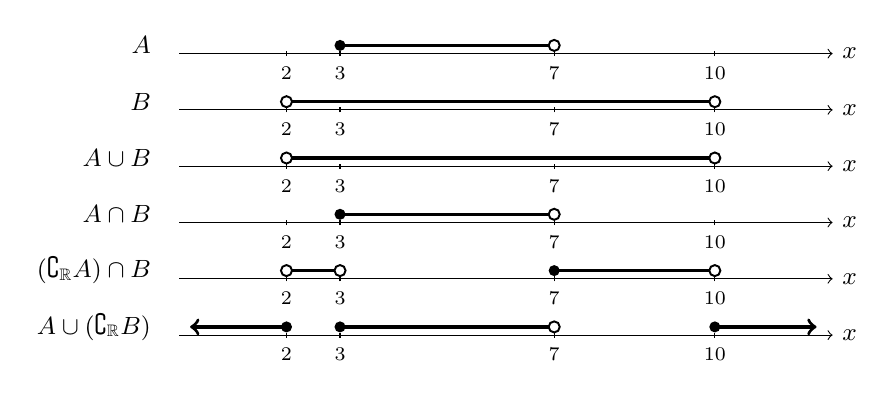
\begin{tikzpicture}[x=0.68cm,y=0.65cm,font=\small]\SetABRows\SetResultRows\end{tikzpicture}\end{center}}
\newcommand{\QuadraticCases}{%
  \begin{center}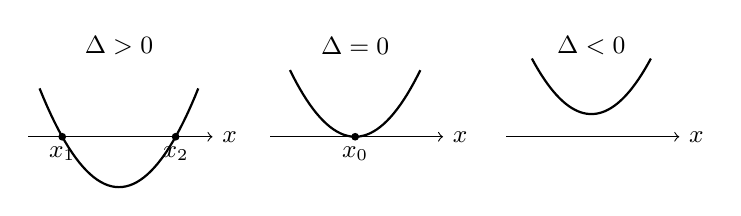
\begin{tikzpicture}[x=0.72cm,y=0.64cm,font=\small]
  \begin{scope}\draw[->] (-1.6,0)--(1.65,0) node[right] {$x$};\draw[thick,domain=-1.4:1.4,samples=45] plot (\x,{\x*\x-1});\fill (-1,0) circle (1.4pt);\fill (1,0) circle (1.4pt);\node[below] at(-1,0){$x_1$};\node[below] at(1,0){$x_2$};\node at(0,1.8){$\Delta>0$};\end{scope}
  \begin{scope}[xshift=3cm]\draw[->] (-1.5,0)--(1.55,0) node[right] {$x$};\draw[thick,domain=-1.15:1.15,samples=40] plot (\x,{\x*\x});\fill (0,0) circle (1.4pt);\node[below] at(0,0){$x_0$};\node at(0,1.8){$\Delta=0$};\end{scope}
  \begin{scope}[xshift=6cm]\draw[->] (-1.5,0)--(1.55,0) node[right] {$x$};\draw[thick,domain=-1.05:1.05,samples=40] plot (\x,{\x*\x+0.45});\node at(0,1.8){$\Delta<0$};\end{scope}
  \end{tikzpicture}\end{center}}

\fancyhead[L]{\small 高一数学期中复习}\fancyhead[R]{\small 考前重点十题}
\begin{document}
\begin{center}{\LARGE\bfseries 高一数学期中复习}\par\vspace{0.2cm}{\Large 考前重点十题}\end{center}
班级\underline{\hspace{2.3cm}}\quad 姓名\underline{\hspace{2.3cm}}\par
请写出必要的文字说明、演算步骤或证明过程。
\Needspace{8\baselineskip}
\textbf{1.}\quad 已知全集为 $\mathbb R$，集合 $A=\{x\mid 3\le x<7\}$，$B=\{x\mid 2<x<10\}$。在数轴上分别表示 $A$、$B$，并求：
\subq{1}$A\cup B$ 与 $A\cap B$；
\subq{2}$(\complement_{\mathbb R}A)\cap B$ 与 $A\cup(\complement_{\mathbb R}B)$。
\SetBlankAxes
\par\vspace*{3.2cm}
\Needspace{8\baselineskip}
\textbf{2.}\quad 解下列不等式：
\subq{1}$2x^2-5x+3<0$；
\subq{2}$-3x^2+x+4\le0$；
\subq{3}$\dfrac{1-2x}{x+2}\ge0$；
\subq{4}$\dfrac{2x-1}{3-4x}\ge1$。
\par\vspace*{4.0cm}
\clearpage
\Needspace{8\baselineskip}
\textbf{3.}\quad 求下列函数的定义域和值域：
\subq{1}$y=2^{2x-x^2}$；
\subq{2}$y=4^x-2^x+1$；
\subq{3}$y=\sqrt{1-2^x}$。
\par\vspace*{4.6cm}
\Needspace{8\baselineskip}
\textbf{4.}\quad 计算或化简下列各式：
\subq{1}$8^{\frac23}+\left(\dfrac{16}{81}\right)^{\frac34}$；
\subq{2}$\left(\dfrac12\right)^{-1}-4\times(-2)^{-3}+\left(\dfrac14\right)^0-9^{\frac12}$；
\subq{3}已知 $a>0$，化简 $\sqrt[3]{a^{\frac32}\sqrt{a^{-3}}}\,\cdot\,\sqrt{(a^{-5})^{-\frac12}\,(a^{-\frac12})^{13}}$；
\subq{4}已知 $-3<x<3$，化简 $\sqrt{x^2-2x+1}-\sqrt{x^2+6x+9}$。
\par\vspace*{4.1cm}
\clearpage
\Needspace{8\baselineskip}
\textbf{5.}\quad 已知 $f(x)=\dfrac{3^x-1}{3^x+1}$。用函数单调性的定义，判断并证明 $f(x)$ 在 $\mathbb R$ 上的单调性。
\par\vspace*{5.7cm}
\Needspace{8\baselineskip}
\textbf{6.}\quad 设 $f(x)=\dfrac{ax-b}{1+x^2}$，$x\in[-1,1]$，其中 $a,b\in\mathbb R$。已知 $f(x)$ 是奇函数，且 $f(1)=-1$。
\subq{1}求 $a,b$ 的值；
\subq{2}写出 $f(x)$，并依据定义证明所得函数是奇函数。
\par\vspace*{5.0cm}
\clearpage
\Needspace{8\baselineskip}
\textbf{7.}\quad 分别解下列不等式：
\subq{1}已知 $f$ 是定义在 $\mathbb R$ 上的偶函数，且在 $[0,+\infty)$ 上严格递增，解 $f(2x-1)<f\!\left(\dfrac13\right)$。
\subq{2}已知 $h$ 是定义在 $[-1,1]$ 上的奇函数，且在 $[-1,1]$ 上严格递减，解 $h(x-1)+h(2x)>0$。
\par\vspace*{5.4cm}
\Needspace{8\baselineskip}
\textbf{8.}\quad 已知 $p(x)$ 是定义在 $\mathbb R$ 上的奇函数，当 $x>0$ 时，$p(x)=x^2-2x+3$。求 $p(x)$ 在 $\mathbb R$ 上的解析式。
\par\vspace*{5.2cm}
\clearpage
\Needspace{8\baselineskip}
\textbf{9.}\quad 求下列函数的最值，并写出取到最值时 $x$ 的值：
\subq{1}$x>1$ 时，$y=x+\dfrac4{x-1}$ 的最小值；
\subq{2}$x<\dfrac54$ 时，$y=4x-2+\dfrac1{4x-5}$ 的最大值。
\par\vspace*{5.1cm}
\Needspace{8\baselineskip}
\textbf{10.}\quad 已知 $a>0$，$b>0$，且 $a+b=2$。求 $\dfrac1a+\dfrac4b$ 的最小值，并写出取到最小值时 $a,b$ 的值。
\par\vspace*{5.9cm}
\end{document}